%%%%%%%%%%%%%%%%%%%%%%%%%%%%%%%%%%%
%%%% INTRODUCCIÓN A LA MEMORIA %%%%
%%%%%%%%%%%%%%%%%%%%%%%%%%%%%%%%%%%

%Buenos días, mi nombre es Miguel González Moreno, soy un antiguo estudiante de la promoción 2014-2019 de ADE+ITI en la Universidad de Deusto. La memoria de mi proyecto de fin de grado la desarrollé en LATEX y a raíz de dicha memoria se ha creado esta plantilla. La plantilla persigue el objetivo de ayudar a cualquier futuro estudiante que se quiera adentrar en este sistema de procesamiento de textos (LATEX). Intentaré explicar cada uno de los campos que aparecen a continuación de modo que todos estén lo más claros posibles y que así, la plantilla, sea de la mayor utilidad posible. Dicho lo cual, comenzamos. 

%Concretamente la memoria y esta plantilla se han realizado en OVERLEAF, un editor de LATEX online pero existen numerosos otros programas que pueden usarse para escribir en este lenguaje. Sin embargo, es posible que algunos de los comandos o funciones cambien de un programa a otro por lo que en caso de cambiar de programa, es probable que algunos comandos no se ejecuten como deberían. En cualquier caso, utilizar otro programa no parece excesivamente complicado pues en caso de que algunos comandos cambien se pueden encontrar fácilmente los equivalentes por Internet. Es cuestión de dedicarle un poco más de tiempo.

%Lo primero de todo, dejar claro que en absoluto soy un experto, es más, ni si quiera soy principiante. Todo lo incluido en esta plantilla se ha aprendido desde cero y lo más probable es que aquello que no está en la plantilla (o que pudiese estar hecho de mejor forma) no lo está puesto que actualmente desconozco como hacerlo, y no porque LATEX no pueda, ya que lo más seguro es que sí se pueda realizar. Así, explicaré todo aquello que sepa dejándoles de profundización en ciertas cuestiones a ustedes. Aquello que desconozca me limitaré a no comentarlo.

%Como se puede observar al compilar, estos textos que aparecen en azul no se escriben en el documento, son comentarios. Los comentarios no son procesados sin embargo sí que se pueden leer en la pantalla de escritura. Intentaré explicar el proceso de creación de la memoria a partir de estos comentarios, siendo todos ellos suprimibles en cuanto el alumno haya comprendido la idea detrás de cada uno de ellos.

%Aún así, si existiese cualquier duda con respecto a la plantilla o a las funciones utilizadas, mi única y principal fuente de conocimiento ha sido Internet, y los maravillosos (y diversos) blogs que se encuentran en la red. Os dejo a continuación aquellos que más me han servido de ayuda (pero la verdad es que hay infinidad). Cualquier función que busquéis, existe. Cualquier problema, lo ha tenido antes otra persona y ha preguntado por ello. Simplemente hay que tener tiempo para encontrar la fuente e ir probando. Esto es prueba y error. 

%Blogs de utilidas: 
%http://minisconlatex.blogspot.com/
%https://tex.stackexchange.com/
%http://metodos.fam.cie.uva.es/~latex/index.html

%Consejo: Por lo general, buscad la ayuda en inglés, hay muchísima más información.

%Finalizada la presentación de la plantilla ¡EMPEZAMOS CON LATEX!

%%%%%%%%%%%%%%%%%%%%%%%%%%%%%%%%
%%%% INTRODUCCIÓN AL LATEX %%%%%
%%%%%%%%%%%%%%%%%%%%%%%%%%%%%%%%

%La escritura en LATEX muy sencilla (una vez se domine lo básico) pero es necesario invertir tiempo para comprenderla, para conocer las funciones y sobre todo para profundizar en ella. Lo básico se aprende rápido. ¡Vamos a ello!

%LATEX trabaja con funciones, todas aquellas palabras que aparecen en verde y van precedidas por el símbolo "\". Cada función suele tener una serie de parámetros opcionales, que se encuentran dentro de "[corchetes]", y una serie de parámetros obligatorios, que se encuentran dentro de "{llaves}". Lógicamente, siempre habrá que introducir un parámetro obligatorio. Los parámetros opcionales se añaden para modificar o precisar elementos de la función en cuestión (dependiendo del uso que le quiera dar el autor).

%En general hay unas funciones básicas que se pueden llamar por defecto, sin embargo para otras es necesario cargar/incluir algunos paquetes especiales. Lo veremos a posteriori (simplemente tenerlo en cuenta).

%%%%%%%%%%%%%%%%%%%%%%%%%
%%%% PRIMERA FUNCIÓN %%%%
%%%%%%%%%%%%%%%%%%%%%%%%%

\documentclass[a4paper,openright,10pt]{book}

%Esta es la primera función del archivo y define el tipo de documento sobre le que se está trabajando. Realmente no tengo un conocimiento exhaustivo sobre los diferentes tipos de documentos en los que se puede trabajar pero encontrar información sobre esta función es muy sencillo.  En este caso, el tipo utilizado es "Book". Se ha utilizado este tipo porque es el más adecuado a documentos largos, con capítulos, secciones y demás. Hay otras clases de documentos como por ejemplo "article", "report" o "memoir". Cada uno con sus características propias. 

%El tipo book permite llamar a otros archivos etcétera. ¿A qué me refiero con llamar a archivos? Como veis en la izquierda estamos trabajando sobre un archivo ".tex" denominado "MAIN.tex". Este archivos es el cuerpo central de nuestra memoria, sin embargo, en él no escribiremos todos los capítulos sino que los capítulos los escribiremos en otros archivos ".tex" (1.Intro.tex, 2.Objetivos.tex y sucesivos) y se llamarán desde "MAIN". Lo veremos más adelante, no os preocupéis. Esto es simplemente para llevar un mayor orden en el documento. Se podría perfectamente escribir toda la memoria en este mismo archivo pero sería algo más caótico y tardaría demasiado en cargar.

%Esta función presntada tiene varios parámetros adicionales: "a4paper", el cual indica que el folio será del tamaño A4, "openright", el cual es utilizado para garantizar que los capítulos nuevos siempre empiecen en una página de la derecha (si en algún momento fuesen a empezar en una página izquierda, LATEX dejará una página en blanco para garantizar esta regla), "10pt" indica el tamaño predeterminado de la fuente a utilizar. 

%Se han indicado así 3 parámetros adicionales. Si no se indican todos los que hay LATEX cogerá los parámetros por defecto en su configuración. Así, que únicamente se hayan indicado 3 no significa que sólo haya 3, probablemente hay muchos más en los que sí se quiere, se puede profundizar buscando información.

%%%%%%%%%%%%%%%%%%%%%%%%%%%%%%%%
%%%% DEFINICIÓN DE PAQUETES %%%%
%%%%%%%%%%%%%%%%%%%%%%%%%%%%%%%%

%LATEX, como se comentaba, no tiene cargadas todas las funciones por defecto (viene lo básico, pero se puede profundizar tanto como se quiera). Así, para ejecutar algunas funciones o símbolos es necesario que se incluyan algunos PAQUETES adicionales. Aquellos en los que se indica PAQUETEB son paquetes prácticamente de inicio, que toda memoria debería como mínimo tener (el resto varía según las necesidades de cada autor).

%Los paquetes se cargan con la función "\usepackage" y aquellos que se han utilizado en la memoria son los siguientes:

\usepackage[utf8]{inputenc}
%PAQUETEB para incluir acentos al escribir en Castellano.
\usepackage[spanish,es-tabla]{babel}
%PAQUETEB para escribir en castellano.
\usepackage{fancyhdr}
%PAQUETEB para definir encabezado y pie de páginas.
\usepackage{ragged2e}
%PAQUETEB utilizado para alinear, justificar o centrar el texto de la memoria.
\usepackage{setspace}
 %PAQUETEB para delimitar el interlineado del texto.
\usepackage{cite}
%PAQUETEB para citar y referencia a lo largo del texto.
\usepackage{enumerate} 
%PAQUETEB para formar listas organizadas y darles formato. 
\usepackage[font={color=RBlue},figurename=Fig.]{caption} 
%Paquete para poner subtítulos a las imágenes y concretamente personalizado para que sean de colo azul (elección personal).
\usepackage{graphicx} 
%Paquete para utilizar distintos colores tanto en la escritura, como en tablas, títulos y demás.
\usepackage{subfigure} 
%Paquete para incluir sub-figuras.
\usepackage{hyperref} 
%Paquete para incluir hyperlinks en el PDF.
\usepackage{eurosym} 
%Paquete para incluir el símbolo "€" en el texto.
\usepackage{pdfpages} 
%Paquete para incluir PDFs a lo largo de la memoria, y modificar su formato.
\usepackage{multirow, array} 
%Paquete para dar formato a las tablas.
\usepackage{float} 
%Paquete para forzar que una foto se introduzca exactamente en un sitio determinado y que LATEX no la reposicione.
\usepackage{longtable} 
%Paquete para la gestión y el formateo tablas de mayor dimensión.
\usepackage{xcolor,colortbl} 
%Paquete para crear colores específicos según RGB.
\usepackage{geometry}
%Paquete para definir las dimensiones de los márgenes.

\definecolor{RBlue}{RGB}{23,33,110} 
\definecolor{Rojo}{RGB}{255,0,0}
\definecolor{Cyan}{RGB}{214,234,240}
\definecolor{Naranja}{RGB}{255,222,199}
\definecolor{GrisTabla}{RGB}{245,245,245}
%Ejemplo de funciones para definir colores a utilizar el documento, según sus dígitos RGB.

%Paquetes para algoritmos matemáticos
\usepackage{amsmath}
\usepackage{algorithm}% http://ctan.org/pkg/algorithms
\usepackage[noend]{algpseudocode}
\makeatletter
% Reinsert missing \algbackskip
\def\algbackskip{\hskip-\ALG@thistlm}
\makeatother

%%%%%%%%%%%%%%%%%%%%%%%%%%%%%%%%%%%%%%%%%%%%%%%%%%%%%%%%%%%
%%%% PROPIEDADES DEL DOCUMENTO (Funciones específicas) %%%%
%%%%%%%%%%%%%%%%%%%%%%%%%%%%%%%%%%%%%%%%%%%%%%%%%%%%%%%%%%%

\setcounter{secnumdepth}{5} 
%Esta función permite que en el índice se indique hasta el sub-nivel número tres. Es decir que aparezcan hasta los apartados 1.1.1. Si se indicase {4}, se podrían observar hasta los sub-apartados 1.1.1.1. 

\setlength{\headsep}{0.5in} 
%La función "\setlength" permite cambiar (sobrescribir valores predeterminados) todas las distancias del documento. En función de que {parámetro} se indique se cambiará una distancia u otra. En este caso se está cambiando la distancia entre el encabezado y el texto para que esta sea durante todo el documento media pulgada. Se puede indicar la distancia que se quiera (cuestiones estéticas) y también se puede indicar la distancia en el sistema métrico (mm, cm).

\onehalfspace 
%Esta función determina que el interlineado a lo largo del documento sea de 1.5. Existen otras funciones para cambiar el interlineado como "\Doublespacing" para interlineado doble, "\singlespace" para interlineado sencillo o "\setspace{}" para indicar aquel que sea preferido de forma específica.

\setlength{\parindent}{0cm}
%Nuevamente se utiliza esta función para cambiar distancias del documento. Concretamente, en este caso se utiliza para cambiar la distancia de las sangrías al comenzar nuevo párrafo. Al marcar el valor en 0, se eliminan las sangrías del documento. Siempre se puede en momentos posteriores forzar la inclusión de alguna sangría o reescribir de nuevo el valor para indicar que a partir de ahí, comiencen las sangrías de nuevo.

\includeonly{
                Chapters/0.Resumen, 
                Chapters/0.Abstract, 
                Chapters/1.Intro, 
                Chapters/3.Objetivos_y_Alcance, 
                Chapters/Funciones,
                Algorithms/ConsensoMath
}
%Esta función es de gran importancia. Como se puede observar a la izquierda, hay una carpeta que se ha creado con diferentes capítulos. Estos capítulos son los diferentes apartados de la memoria en los que se va a ir escribiendo. Por ejemplo, el capítulo de la introducción, el capítulo de objetivos, el capítulo de la memoria técnica, o el capítulo del plan de trabajo. Bien, de cara a poder incluirlos a posteriori en esto documento principal (MAIN.tex) es necesario indicarle a LATEX que los cargue y eso se realiza con esta función. Así, habrá que incluir tantos parámetros como capítulos se deseen cargar. Los parámetros son simplemente la dirección de la carpeta en la que se encuentran, y su nombre.

\geometry{top=3cm, bottom=3cm, left=3.5cm, right=2.5cm}
%Esta función determina los márgenes que se han de utilizar a lo largo de todo el documento. Así, el margen superior será de 3 centímetros, igual que el inferior y los márgenes exterior e interior serán de 3.5 y 2.5 centímetros respectivamente.

\pagestyle{empty}
%Esta función es bastante útil ante diversos problemas que puedan surgir a lo largo del documento con las páginas en blanco. Esta función determina que el estilo (encabezados y pies de página) de la página estrictamente posterior sea totalmente blanco (vacío - empty).

%%%%%%%%%%%%%%%%%%%%%%%%%%%%%%%%%%%%%%%%%%%%%%%%%%%%%%%%%%%%%%%%
%%%% COMIENZA EL DOCUMENTO (con la función \begin{document} %%%%
%%%%%%%%%%%%%%%%%%%%%%%%%%%%%%%%%%%%%%%%%%%%%%%%%%%%%%%%%%%%%%%%

\begin{document}

%%%%%%%%%%%%%%%%%%%%
%%%% PAGINACIÓN %%%%
%%%%%%%%%%%%%%%%%%%%

\pagestyle{fancy}
%Esta función es utilizada para crear un nuevo estilo de formato, es el formato "fancy". En él vamos a determinar a continuación cómo se quieren posicionar pies de página, encabezados y demás.

\lhead{}
%Esta función sirve para que no se escriba nada (parámetro obligatorio vacío) en el encabezado en la posición izquierda. 

\chead{}
%Esta función sirve para que no se escriba nada (parámetro obligatorio vacío) en el encabezado en la posición central. 

\rhead{}
%Esta función sirve para que no se escriba nada (parámetro obligatorio vacío) en el encabezado en la posición derecha. 

\cfoot{}
%Esta función sirve para que no se escriba nada (parámetro obligatorio vacío) en el pie de página en la posición central. 

\fancyhead[OR]{}
%Esta función sirve para que no se escriba nada (parámetro obligatorio vacío) en el las páginas impares, en el encabezado en la posición derecha.

\fancyhead[OL]{}
%Esta función sirve para que no se escriba nada (parámetro obligatorio vacío) en el las páginas impares, en el encabezado en la posición izquierda.

\fancyhead[ER]{}
%Esta función sirve para que no se escriba nada (parámetro obligatorio vacío) en el las páginas pares, en el encabezado en la posición derecha.

\fancyhead[EL]{}
%Esta función sirve para que no se escriba nada (parámetro obligatorio vacío) en el las páginas pares, en el encabezado en la posición izquierda.

\fancyfoot[LE,RO]{\thepage} 
%Esta función sirve para indicar que el número de la página correspondiente se escriba a la izquierda en las páginas pares y a la derecha en las páginas impares.

\renewcommand{\headrulewidth}{0pt} 
%Esta función sirve para renovar todo tipo de comandos o distancias en el documento. Concretamente, en este caso se indica que no exista (grosor 0pt) una linea debajo del encabezado que lo separe del texto.


\includepdf[]{PDF/Portada_TFG_IngenieriaInformatica}
%Esta función incluye el PDF de la portada correspondiente al TFG. Dicho documento PDF ha de estar cargado en el menú de la izquierda como se encuentra esta portada auxiliar. Es importante incluir en el parámetro obligatorio la dirección a dicho PDF con su normbre correspondiente.

\newpage
\thispagestyle{empty}


\frontmatter
%Esta función sirve para que, en las primeras páginas de la memoria (hasta que se indique lo contrario con otra función), la paginación sea en números romanos como lo indican los criterios de formato en índice, resumen y demás apartados.

%como se puede ver, todo lo expuesto arriba (en términos de paginación) es un poco redundante y bastante lioso, aún así, funciona. Ahora, no tengo ninguna duda de que se puede optimizar, eliminar funciones o sustituir por otras para que sea más "user-friendly". Estaré encantado de escuchar como hacerlo, pero de momento desconozco como mejorar el código sin que genere errores. Dicho esto, como se comentaba al principio, es cuestión de dedicarle  tiempo y comprender más a fondo las funciones. 

\setcounter{page}{3}
%Esta función permite comenzar el contador de las páginas para la numeración en el número 3, es importante puesto que los primeros números van dedicados a portada y contraportada y no se numeran. Así, la primera página numerada será la 3. 

\chapter*{Resumen}
%Esta función determina el comienzo de un nuevo capítulo. El parámetro indica el título de lo que será el capítulo. Hay dos funciones que inician un nuevo capítulo "\Chapter*" y "\Chapter", con asterisco y sin él. El asterisco se utiliza para que no sea vea: "Capítulo 1: Resumen" y únicamente se vea "Resumen" (Gustos personales).

\thispagestyle{fancy}
%Como ya se ha visto anteriormente, esta función determina que en las páginas se utilice el estilo fancy (previamente creado). Este estilo no tiene ningún encabezado (como se ha determinado) y sólo incluye los números de página en los pies de página correspondiente (izquierda o derecha).

%%%%%%%%%%%%%%%%%%%%%%%%%%%%%%%%%%%%%%%%%%%%%%%%%%%%%%
%%% A continuación, al final, COMENZAMOS A ESCRIBIR%%% 
%%%%%%%%%%%%%%%%%%%%%%%%%%%%%%%%%%%%%%%%%%%%%%%%%%%%%%


%En LATEX se escribe igual que en cualquier otro procesador de texto, y en este caso sin los símbolos de "%" que estoy utilizando actualmente y que generan comentarios explicativos.%

Lorem ipsum dolor sit amet, consectetur adipiscing elit. Aenean semper non orci at fringilla. Etiam fermentum in diam vestibulum pellentesque. Nam volutpat, velit ut euismod mollis, ipsum erat facilisis justo, et tempor est lectus nec massa. Pellentesque habitant morbi tristique senectus et netus et malesuada fames ac turpis egestas. Sed accumsan viverra neque eu blandit. Suspendisse in fermentum felis, id iaculis mi. Quisque maximus quam lacus, non lobortis libero tincidunt at. Pellentesque habitant morbi tristique senectus et netus et malesuada fames ac turpis egestas. Maecenas lectus nibh, sagittis ut felis non, fermentum ullamcorper leo. In hac habitasse platea dictumst. Orci varius natoque penatibus et magnis dis parturient montes, nascetur ridiculus mus. Fusce est dui, dapibus ultricies ipsum quis, ultrices maximus dolor. Proin finibus, lorem vulputate maximus convallis, quam tellus posuere magna, sed maximus nunc eros quis ipsum. Cras dignissim cursus lectus ac auctor. Donec suscipit vestibulum neque, sed lobortis est rhoncus non.\\

Praesent ut neque eros. Praesent vitae augue at diam tincidunt sagittis. In cursus lorem nec neque condimentum dictum. Morbi vel tristique orci. Cras luctus tempus elit tincidunt hendrerit. Proin bibendum arcu et sapien finibus vulputate sed eget leo. Duis at bibendum massa, sit amet ornare lorem. Donec dictum finibus fringilla. Duis accumsan lectus dolor, eu maximus ligula semper vel. Proin a sem tincidunt, mollis magna eget, consequat tortor. In sodales justo et varius scelerisque. Aliquam sit amet lacus mollis, tincidunt erat vitae, lacinia sem. Maecenas vel erat sagittis, semper ex in, commodo libero.\\

Integer malesuada quis elit eu eleifend. Suspendisse non vestibulum est, a fermentum urna. Donec ligula tortor, ultrices varius nisi eget, dictum malesuada augue. Fusce lacus orci, eleifend quis luctus dictum, ultricies id turpis. Vestibulum et auctor orci. Pellentesque habitant morbi tristique senectus et netus et malesuada fames ac turpis egestas. Integer facilisis neque quis dui dapibus dictum.\\

%IMPORTANTE: LATEX no tiene en cuenta si en el código que habéis escrito ponéis un único espacio entre las palabras o como yo ahora,    256              espacios. LATEX lo procesará como si existiese un único espacio. 




%Lo mismo ocurre con los "intros" para cambiar de párrafo, da igual cuantos escribáis a mano, LATEX interpretará como si sólo hubiera uno. También habréis podido deducir que el "intro" no se escribe con la tecla clásica sino mediante la escritura de dos "\\" al final de cada párrafo.

\textbf{Descriptores}\\
Lorem, ipsum, dolor, sit, amet


\newpage
%Función para incluir un salto a una nueva página.
\thispagestyle{empty}
%Función para que dicha página no tenga ningún formato (ni número, ni encabezado).

%Así con estas dos funciones de forma consecutiva se crea una página en blanco.
\chapter*{Abstract}
%Nuevo capítulo para incluir el resumen (si se quiere también en inglés).

\thispagestyle{fancy}
Lorem ipsum dolor sit amet, consectetur adipiscing elit. Aenean semper non orci at fringilla. Etiam fermentum in diam vestibulum pellentesque. Nam volutpat, velit ut euismod mollis, ipsum erat facilisis justo, et tempor est lectus nec massa. Pellentesque habitant morbi tristique senectus et netus et malesuada fames ac turpis egestas. Sed accumsan viverra neque eu blandit. Suspendisse in fermentum felis, id iaculis mi. Quisque maximus quam lacus, non lobortis libero tincidunt at. Pellentesque habitant morbi tristique senectus et netus et malesuada fames ac turpis egestas. Maecenas lectus nibh, sagittis ut felis non, fermentum ullamcorper leo. In hac habitasse platea dictumst. Orci varius natoque penatibus et magnis dis parturient montes, nascetur ridiculus mus. Fusce est dui, dapibus ultricies ipsum quis, ultrices maximus dolor. Proin finibus, lorem vulputate maximus convallis, quam tellus posuere magna, sed maximus nunc eros quis ipsum. Cras dignissim cursus lectus ac auctor. Donec suscipit vestibulum neque, sed lobortis est rhoncus non.\\

Praesent ut neque eros. Praesent vitae augue at diam tincidunt sagittis. In cursus lorem nec neque condimentum dictum. Morbi vel tristique orci. Cras luctus tempus elit tincidunt hendrerit. Proin bibendum arcu et sapien finibus vulputate sed eget leo. Duis at bibendum massa, sit amet ornare lorem. Donec dictum finibus fringilla. Duis accumsan lectus dolor, eu maximus ligula semper vel. Proin a sem tincidunt, mollis magna eget, consequat tortor. In sodales justo et varius scelerisque. Aliquam sit amet lacus mollis, tincidunt erat vitae, lacinia sem. Maecenas vel erat sagittis, semper ex in, commodo libero.\\

Integer malesuada quis elit eu eleifend. Suspendisse non vestibulum est, a fermentum urna. Donec ligula tortor, ultrices varius nisi eget, dictum malesuada augue. Fusce lacus orci, eleifend quis luctus dictum, ultricies id turpis. Vestibulum et auctor orci. Pellentesque habitant morbi tristique senectus et netus et malesuada fames ac turpis egestas. Integer facilisis neque quis dui dapibus dictum.\\

\textbf{Descriptors}\\
Lorem, ipsum, dolor, sit, amet


\newpage
\thispagestyle{empty}

\fancypagestyle{plain}
{
}
%Se define mediante esta función el formato plain, que no tiene nada, ni encabezados ni pies de página. Realmente esta función podría ir a comienzo del documento o en cualquier lugar, es decir, se puede mover.

\tableofcontents
%Esta función permite introducir el índice de capítulos (hasta el subíndice que se haya indicado previamente).

\newpage
\thispagestyle{empty}

\cleardoublepage
%Esta función permite que aunque acabe en página impar, el siguiente apartado, comience en página impar. Con este comando te aseguras que se hace bien y que además se mantiene la numeración correspondiente en números romanos. Es decir, la página que se quedaría en blanco no está en blanco sino que mantiene la numeración. En caso de no querer numeración hay que utilizar los comando ("\newpage" y "\thispagestyle{empty}).

\newpage
\thispagestyle{empty}

\listoffigures
% Es la función que introduce el índice de figuras. Funciona exactamente igual que el de capítulos.
\newpage
\thispagestyle{empty}

\cleardoublepage

\listoftables
%Por ultimo, se introduce el índice de tablas en caso de que las hubiera en vuestro documento. 

\newpage
\thispagestyle{empty}
%Página en blanco

\mainmatter
%Esta función se utiliza para indicar que a partir de ahora la numeración pasa a ser con números estándar y no con romanos como se había venido utilizando hasta ahora.

\pagestyle{fancy}
%A continuación se vuelve a redefinir el estilo “fancy” para que se adecúe al que ha de utilizarse a lo largo de toda la memoria. El estilo es el siguiente:

\lhead{}
%Encabezado a la izquierda vacío. En realidad debe de ir el nombre del capítulo en el que se está escribiendo pero ello se gestionará dentro de cada capítulo (pues el nombre cambia). Aquí se define el formato general.

\chead{}
%Encabezado en el centro vacío.

\fancyhead[OR]{PROYECTO FIN DE GRADO}
%En el encabezado a la derecha en las páginas pares se escribe: "PROYECTO FIN DE GRADO".

\fancyhead[OL]{} 
%Encabezado a la izquierda en las páginas pares vacío. Probablemente esta función sea redundante con la función \lhead y sería omitible.

\fancyhead[ER]{}
%Encabezado en las páginas impares a la derecha vacío.

\cfoot{} 
% Pie de página en el centro vacío.

\fancyfoot[LE,RO]{\thepage} 
%En el pie de página se va a escribir el número de la página correspondiente. Se escribirá en la derecha en las páginas pares y en la izquierda en las páginas impares.

\renewcommand{\headrulewidth}{0pt} 


%\chapter{Introducción}\label{Int}
%Función que crea el título de capítulo y al cual se le da el nombre deseado a través de su parámetro obligatorio. Al no tener la función el “*” se escribirá también en el título del documento las palabras “Capítulo 1: …”. Además se indica, mediante la función “\label”, la correspondiente etiqueta que lleva asociada. La etiqueta sirve para que en caso de que luego se quiera hacer referencia al capítulo se haga llamando etiqueta tal que se escribiría “La información correspondiente a dicho tema se encuentra en el capítulo \ref{Int}.”

\thispagestyle{fancy}
%Función que determina que durante este capítulo se aplique el estilo Fancy.

\fancyhead[LE]{\thechapter.NOMBRE DEL PRIMER CAPÍTULO} 
%Función que se utiliza para indicar que en las páginas impares, aparezca en el encabezado en la parte izquierda, el número del capítulo con su correspondiente nombre.

Lorem ipsum dolor sit amet, consectetur adipiscing elit. Fusce bibendum mauris metus, quis pellentesque nisl vestibulum ut. Cras finibus, tortor id mattis imperdiet, tellus risus consectetur nisi, et luctus neque nisl nec massa. Sed interdum lacus eget nisl porttitor mattis. Donec volutpat blandit tortor ut porttitor. Integer nec pulvinar sapien. Integer eget odio feugiat, pretium tortor vel, dictum est. Proin ac eleifend augue, vitae facilisis dolor. Suspendisse at augue maximus, maximus est in, posuere dui. Nam id lorem et leo vehicula faucibus. Proin ac nunc sit amet metus ullamcorper fringilla non in quam. Sed at condimentum enim.\\
%Texto sin sentido y predeterminado que se irá utilizando a lo largo de todo el documento para simular la escritura de la memoria.

\setlength{\fboxsep}{5pt}
\begin{figure}[thbp]
\centering
\fbox{
\includegraphics[width=0.6\textwidth, height=3.8cm]{Figuras/LDeusto.jpeg}}
\caption{Logo de Deusto (Fuente: Universidad de Deusto \cite{Deusto}} \label{fig:Deusto}
\end{figure}
%Todas estas funciones aparecen explicadas con detalle en el documento "Funciones.tex".

\textcolor{Rojo}{Como se puede observar en la imagen \ref{fig:Deusto}}: Cras neque purus, vulputate at neque a, rutrum elementum odio. Sed ultrices enim nulla, ac consectetur enim malesuada maximus. Nulla facilisi. Curabitur pharetra tortor nisl, vel molestie turpis commodo eget. Morbi viverra urna varius, condimentum nulla eu, semper mi. Aenean faucibus erat id felis consequat, sit amet porttitor nibh posuere. Proin imperdiet fermentum odio eget aliquet. Aenean quis auctor ante, ut consequat nunc. Maecenas ac lacinia risus. Donec finibus erat in mattis pharetra. Morbi sed metus eget magna luctus placerat quis eget velit. Praesent imperdiet velit ut magna bibendum pretium. Vestibulum fermentum nulla et suscipit tempor. Vestibulum facilisis vulputate faucibus. Vivamus et elementum tellus, at accumsan augue. Fusce elementum sem ut nunc efficitur ullamcorper. Sed ac erat quis massa pellentesque gravida id sit amet nulla. Nunc ultricies porttitor metus at fermentum \cite{Deusto}.\\

\setlength{\fboxsep}{0pt}
%"\Fbox" es una función que como se verá posteriormente es utilizada para recuadrar fotos o enmarcarlas con un borde negro. Esta función indica que no haya separación entre la foto y el marco, es decir, que justo aparezca el marco cuando acabe la foto. Se puede cambiar el "0pt" por otro número y se dejará un espacio alrededor de la foto hasta que comience el marco.

\begin{figure}[H]
\centering
\begin{minipage}[h]{.48\linewidth}
\vspace{1.5cm}
\centering
\fbox{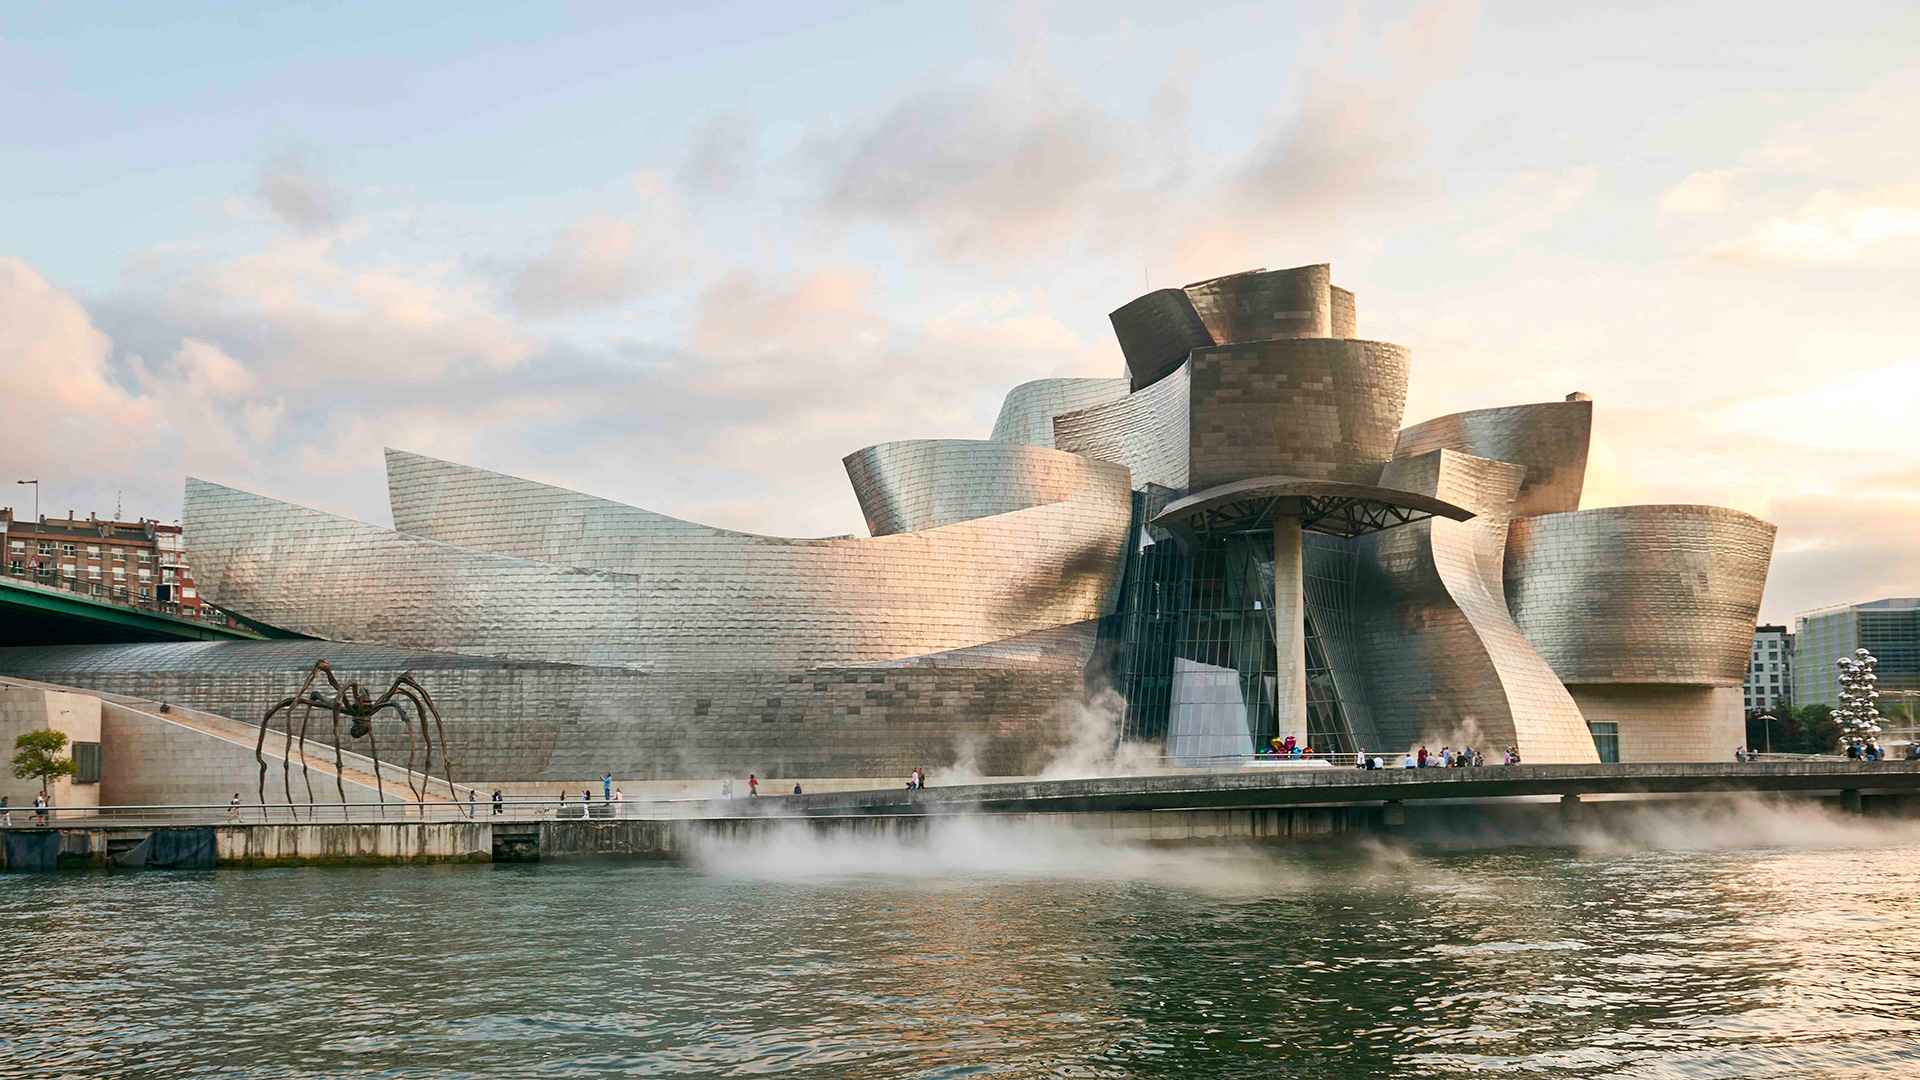
\includegraphics[width=\textwidth, height=4.5cm]{Figuras/Gugg.jpg}}
\caption{Guggenheim - Bilbao (Fuente: Google \cite{Gugg}).} \label{fig:Gugg}
\end{minipage}
\hfill
\begin{minipage}[h]{.45\linewidth}
\centering
\fbox{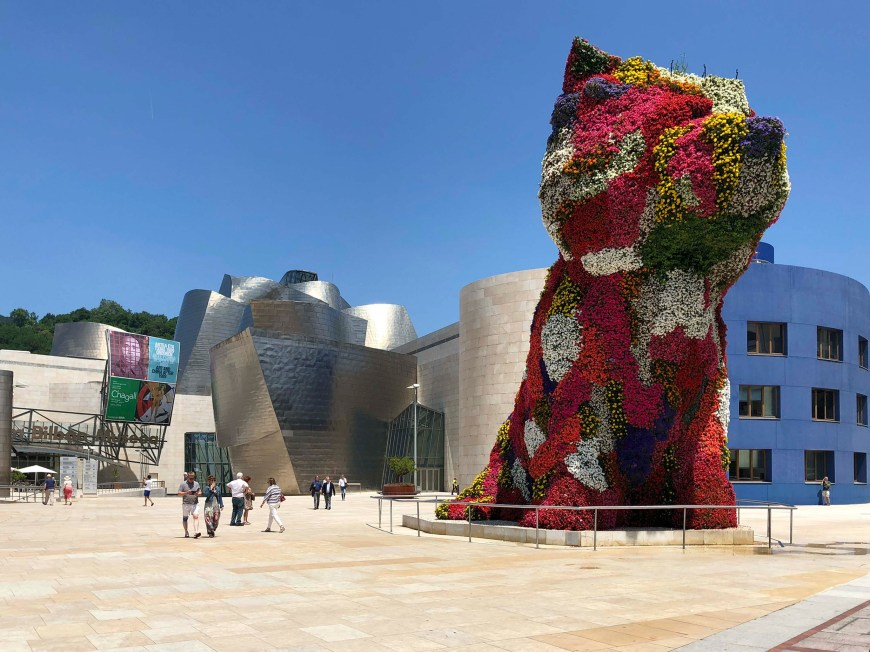
\includegraphics[width=\textwidth, height=6cm]{Figuras/Puppy.jpg}}
\caption{Puppy - Guggenheim (Fuente: Google \cite{Puppy}).} \label{fig:Puppy}
\end{minipage}
\end{figure}

Cras efficitur purus ut ante sollicitudin, vel vulputate enim pulvinar. Suspendisse sit amet erat ut dui accumsan pharetra eget in arcu. Vestibulum fermentum a velit ac cursus. In tempus elit risus, a vestibulum est viverra a. Vestibulum ut nulla venenatis, congue urna quis, ullamcorper lacus. Duis ac hendrerit nisi, id imperdiet purus. Proin non iaculis sem. Suspendisse potenti. Nulla sed dui orci. Pellentesque vel feugiat quam, non eleifend purus. Donec porttitor velit vel sollicitudin cursus. Vivamus rhoncus vel risus non vestibulum. Aenean fermentum congue pretium. Donec dolor felis, iaculis iaculis gravida vitae, placerat ac enim.

\section{Sección}
Etiam interdum lectus nec elementum consequat. Maecenas at enim et ante aliquet porta pellentesque vitae libero. Integer tortor magna, efficitur in mauris vel, cursus consectetur magna. Donec nec nibh ultricies, ultricies velit interdum, porta nibh. Curabitur ornare, ex nec finibus interdum, leo felis semper dui, vitae auctor velit libero at arcu. In hendrerit tortor quis tempus efficitur. Aenean vel feugiat nisi, quis sagittis ex. Duis sit amet blandit ligula. Curabitur quis enim nibh. Nulla facilisi. Nunc nec dictum libero. Sed mattis euismod nulla et bibendum.

\begin{itemize}
\renewcommand{\labelitemi}{$\bullet$}
\setlength{\itemindent}{5mm}
    \item Curabitur ullamcorper varius congue.
    \item Vivamus eu quam sem. Aenean a ligula a est blandit dignissim vel non odio.
    \item Etiam sit amet velit quis enim porta semper sit amet vitae diam.
\end{itemize}

\subsection{Subsección}
In bibendum urna libero, ut maximus ex pharetra non. Aliquam sed metus eget lacus suscipit bibendum eget sed risus. Aenean dictum, urna eu lobortis auctor, quam sem porta ex, ut dignissim lectus sapien et dui. Phasellus eros massa, imperdiet vitae elit et, malesuada feugiat odio. Vivamus interdum turpis sit amet ligula rhoncus semper. Curabitur nec consequat libero, at suscipit neque. Donec commodo arcu vel eros feugiat, vitae hendrerit risus efficitur. Nulla convallis ex sed nisi ullamcorper feugiat.\\

\renewcommand{\arraystretch}{1.6}
\begin{table}[]
\begin{center}
\begin{tabular}{|m{7cm}| m{7cm} |}
\hline
\rowcolor{Cyan}
\centering \textbf{Lorem ipsum} & \hspace{2.75cm} \textbf{Dolor sit} \\\hline
\textbf{Consectetur adipiscing} & Elit\\ \hline
\rowcolor{GrisTabla}
\textbf{Consectetur adipiscing} & Elit \\ \hline
\textbf{Consectetur adipiscing} & Elit \\ \hline
\rowcolor{GrisTabla} 
\textbf{Consectetur adipiscing} & Elit \\ \hline
\rowcolor{Naranja} 
\textbf{In bibendum urna} & \textbf{Libero} \\ \hline
\end{tabular}
\caption{Tabla con texto por defecto (Fuente: Elaboración propia).}
\label{Medioambiente}
\end{center}
\end{table}

\subsubsection{Subsubsección}

Lorem ipsum dolor sit amet, consectetur adipiscing elit. Phasellus scelerisque sem quis sem commodo dictum. Maecenas venenatis hendrerit tortor, eget maximus dui ultrices ac. Vivamus aliquam ipsum non tellus lacinia varius. Nunc dapibus porta commodo. Praesent et porttitor nibh. Nunc consectetur congue dolor, ut venenatis leo. Suspendisse potenti. Nunc non nisi a metus vestibulum euismod. Vivamus dapibus lobortis sagittis. Fusce tincidunt neque velit, sed gravida ex interdum vel.\\

Ut commodo suscipit aliquet. Phasellus accumsan rhoncus lectus sit amet blandit. Duis nec quam et sapien blandit volutpat. Pellentesque nec nisl non tellus aliquet facilisis. Quisque dictum arcu quis leo blandit pulvinar non non nisi. Vivamus accumsan nec enim at scelerisque. Vestibulum ante ipsum primis in faucibus orci luctus et ultrices posuere cubilia Curae; Suspendisse hendrerit tellus ut massa sagittis, in pellentesque odio pulvinar. Sed tristique viverra mi, vitae ornare orci vestibulum eu. Nunc quis elit ante.\\
\newpage
\thispagestyle{empty}
\chapter{Objetivos y Alcance}\label{Obj}
\thispagestyle{fancy}
\fancyhead[LE]{\thechapter.Objetivos y Alcance} 
\section{Obejetivos}
Los objetivos de este proyecto pueden clasificarse en varios grupos. Por un lado están los objetivos generales, objetivos que a simple vista no tienen hitos específicos para en qué estado se encuentran y si se han cumplido o no.
\\\\
Por otro lado se encuentran los objetivos específicos, estos, al contrario que los generales, son hitos específicos fácilmente identificables que permiten saber si la tarea se ha completado, y en caso contrario saber en qué estado se encuentra la tarea. Dentro de este grupo se encuentran los objetivos específicos de desarrollo, apartado donde se agrupan los objetivos que permiten saber en qué estado de desarrollo se encuentra el proyecto y que funcionalidades incorpora. Pero además, también se encuentran los objetivos de estudio, donde se incluyen los objetivos que tienen que ver con el estudio de los diferentes experimentos que se realizarán. 

\subsection{Generales}
El objetivo general de este proyecto es el de desarrollar un sistema de recomendaciones online basado en federated learning. Este sistema se desarrollará sobre un sistema de recomendaciones ya existente basado en Machine Learning y deberá adaptarlo para su correcto funcionamiento con información descentralizada.
\\ \\
Para respetar la privacidad y derechos de los usuarios el proyecto deberá incluir la privacidad como patrón de diseño, cumpliendo tanto con las normativas vigentes en Europa y España,como con las posibles nuevas medidas que entren en vigor en un futuro. 
\\ \\
Por último, el sistema deberá asegurar que la información se quede en el dispositivo y no se comparta ninguna información que no sea la del propio modelo desarrollado por el participante de la red.

\subsection{Específicos}
Los objetivos específicos son fácilmente reconocibles y concretos, lo que permite saber con exactitud cuando se han cumplido los objetivos y cuando no.

\subsubsection{De desarrollo}
Los objetivos de desarrollo tienen que ver con el correcto desarrollo del sistema de recomendación basado en federated learning.
\\ \\
\textbf{Formación: }
El alumno deberá formarse en conocimientos sobre Inteligencia Artificial para poder comprender los conceptos. También deberá familiarizarse con el código del sistema de recomendación para realizar las modificaciones pertinentes.
\\ \\
\textbf{Parametrización y configuración: }
Se tendrán que configurar las plataformas de desarrollo para poder ejecutar el sistema de recomendación centralizado con mayor rapidez y agilizar el desarrollo del proyecto. También se tendrán que configurar las Raspberries y la Jetson Nano, aprovisionarlas del software necesario para ejecutar en ellas el sistema de recomendación y ejecutarlo sin problemas.
\\ \\
\textbf{Sistema de recomendación: }
Se deberá hallar la forma de combinar modelos de IA de cada Raspberry y se realizarán las modificaciones pertinentes en el sistema de recomendación para cumplir los siguientes puntos:
\begin{itemize}
    \item Que sea capaz de obtener las recomendaciones para un único usuario en concreto. 
    \item Que sea capaz de guardar y cargar los modelos entrenados de LightFM.
    \item Que el modelo de LightFM sea capaz de admitir aprendizaje incremental.
\end{itemize}

\subsubsection{De estudio}
Los objetivos de estudio tienen que ver con el análisis de los resultados del sistema de recomendación basado desarrollado sobre federated learning.
\\ \\
\textbf{Análisis: }
El estudio del sistema deberá analizar la diferencia de rendimiento entre el sistema de recomendación con información centralizada y distribuida. Y analizar cómo afectan los distintos modelos y su combinación al rendimiento del sistema de recomendación.
\\ \\
\textbf{Privacidad: }
Hay que valorar y analizar la privacidad y seguridad de los datos personales de los usuarios tanto en el modelo central, como en el distribuido. Se deberán evitar los problemas de seguridad y privacidad implícitos de la implementación de un sistema de recomendación basado en federated learning

\section{Alcance}
En el alcance se centra en concretar qué objetivos entran en el desarrollo del proyecto y cuáles no. Para ello se ha dividido este apartado en dos grupos, los objetivos y tareas que entran en el alcance del proyecto y los que no. La segregación en estos grupos nos permite concretar con más precisión los límites del proyecto, evitando que el proyecto se amplíe más allá de sus límites. 
\\ \\
\subsection{Dentro del alcance}
Entran dentro del alcance los objetivos y tareas derivadas del desarrollo de un sistema de recomendación basado en federated learning, tanto las tareas de parametrización y configuración del hardware como el desarrollo de software. Esto incluye todos los objetivos específicos de desarrollo mencionados en el apartado anterior.
\\ \\
También se incluye el estudio y análisis de los resultados del sistema de recomendación, así como su precisión y sus inconvenientes, es decir, todo lo comentado en los objetivos específicos de estudio.
\\ \\
Para finalizar se incluirá un estudio de la estabilidad legal del sistema en el tiempo. Esto incluye la corroboración del cumplimiento de las actuales medidas de protección de datos y el estudio de las posibles futuras medidas, legislaciones y derechos que limiten el uso de información en Europa.
\\ \\
Todo esto quedará recogido en la memoria técnica del proyecto que será entregada como proyecto fin de grado.

\subsection{Fuera del alcance}
Fuera del alcance queda cualquier estudio de mercado sobre si la solución sería viable económicamente además de cualquier estudio de alternativas a federated learning. 
\\ \\
No se incluirá ni se recogerá ninguna legislación fuera del marco jurídico Español y del Ordenamiento jurídico de la Unión Europea. Lo que deja fuera del alcance cualquier derecho, legislación o restricción de cualquier estado u organización ajeno a los comentados.
\\ \\
Queda fuera del alcance también la encriptación de las comunicaciones entre los diferentes dispositivos.
\\
%Funciones para incluir los otros documentos que se han desarrollado. Dichos documentos son los distintos capítulos de la memoria. Toda la escritura de los mismos se realizará en los documentos de forma específica y no en este archivo “MAIN.tex”. Así que vamos a ellos.


\chapter{Sistema de recomendación}
\thispagestyle{fancy}
\section{LightFM}
LightFM es una implementación en python de varios algotitmos populares de recomendación.
\subsection{Creación del modelo}
El paso de creación del modelo es un paso complejo puesto que conlleva la correcta gestión de muchos datos e información. Asimismo, estos datos han de estar correctamente estructurados y construidos, puesto que LightFM requiere que la información este convertida a matrices dispersas y no tolera elementos vacíos en ellas. Para ello LightFM proveé de herramientas de creación de datasets que facilitan la creación de las matrices, de forma que sea más fácil incluirlas en el modelo. 
\\ \\
Entre estas erramientas se encuentran:

\begin{itemize}
    \item \textit{build\_user\_features($\ldots$)} \quad Permite crear la matriz CSR de usuarios y atributos de usuarios.
    \item \textit{build\_item\_features($\ldots$)} \quad Permite crear la matriz CSR  de items y atributos de items.
    \item \textit{build\_interactions($\ldots$)} \quad Permite crear las matriz COO de interacciones y las matriz COO de sus correspondientes pesos.
\end{itemize}

Hay que tener en cuenta que las matrices CSR (Compressed Sparse Row) hacen referencia a las matrices que admiten operaciones matriciales y acceso eficientemente; y que las matrices COO (Coordinate list) hacen referencia a las matrices que soportan modificaciones eficientemente, son generalmente utilizadas para construir matrices.


\subsubsection{Atributos de los usuario}
Para crear el modelo es necesario, entre otras cosas, disponer de las características de los usuarios. En este caso contamos con multitud de atributos sobre cada usuario: edad, género, nivel educativo, país, cultura de trabajo, perfil PST (Pinball, Shortcut, Thought-ful), barreras, intenciones y confianza.
\\ \\
Para convertir toda esa información del usuario a la matriz CSR que exige LightFM habrá que llamar a \textit{build\_user\_features($\ldots$)} con los IDs de usuario y y sus atributos, formando una lista que tenga listas de los IDs de los usuarios con sus listas de atributos, es decir:
\begin{align*}
    \begin{bmatrix}
        \begin{bmatrix} 
            userId$$_{1}$$ & \begin{bmatrix} feature$$_{11}$$ &\cdots & feature$$_{1w}$$ \end{bmatrix}$$_1$$
        \end{bmatrix}
        &
        \ldots
        &
        \begin{bmatrix} 
            userId$$_{v}$$ & \begin{bmatrix} feature$$_{v1}$$ &\cdots & feature$$_{vw}$$ \end{bmatrix}$$_v$$
        \end{bmatrix}
    \end{bmatrix}
\end{align*}
Teniendo en cuenta que:
\begin{align*}
    \textit{v}\gets & \textit{Cantidad de IDs de usuario }
    &&\\
    \textit{w} \gets & \textit{Contidad de atributos por usuario}
    &&\\
    \textit{userId$_{v}$} \gets & \textit{ID del usuario v}
    &&\\
    \textit{feature$_{vw}$} \gets & \textit{Atributo w del usuario v}
\end{align*}
%
Una vez creada la lista y pasado como parámetro al método, obtendremos la matriz CSR de atributos de usuario.

\subsubsection{Atributos de los elementos}
Además de los usuarios y de sus atributos, también se ha de disponer de los elementos a ordenar en el ranking, llamados items, y de sus características. En este caso estos items representan las estrategias de persuasión por las que se preguntó a los usuarios en el cuestionario. Sin embargo, al contrario que en el punto anterior, no contamos con tantos atributos sobre estos items, sino que cada estrategia de persuasión cuenta con dos atributos llamados dimensiones. Estos atributos no se encuentran presente en todas las estrategias, lo que da como resultado que haya algunas que tengan dos, una o ninguna dimension.
\\ \\
Para convertir toda esa información de los items a la matriz CSR que exige LightFM habrá que llamar a \textit{build\_item\_features($\ldots$)} con los IDs de las estrategias y y sus atributos, formando una lista que tenga listas de los IDs de las estrategias con sus listas de atributos, es decir:
\begin{align*}
    \begin{bmatrix}
        \begin{bmatrix} 
            itemId$$_{1}$$ & \begin{bmatrix} feature$$_{11}$$ &\cdots & feature$$_{1w}$$ \end{bmatrix}$$_1$$
        \end{bmatrix}
        &
        \ldots
        &
        \begin{bmatrix} 
            itemId$$_{v}$$ & \begin{bmatrix} feature$$_{v1}$$ &\cdots & feature$$_{vw}$$ \end{bmatrix}$$_v$$
        \end{bmatrix}
    \end{bmatrix}
\end{align*}
Teniendo en cuenta que:
\begin{align*}
    \textit{v}\gets & \textit{Cantidad de IDs de estrategias }
    &&\\
    \textit{w} \gets & \textit{Contidad de dimensiones por estrategia}
    &&\\
    \textit{itemId$_{v}$} \gets & \textit{ID de la estrategia v}
    &&\\
    \textit{feature$_{vw}$} \gets & \textit{Atributo w de la estrategia v}
\end{align*}
%
Una vez creada la lista y pasado como parámetro al método, obtendremos la matriz CSR de atributos de usuario.
%
%
\subsubsection{Interacciones}


Para crear un modelo de LightFM se necesita

user\_features, item\_features 

model = LightFM() 

% model.fit(train\_interactions,
%         user\_features=user\_features,
%         sample\_weight=train\_weights,
%         epochs=100,
%         num\_threads=4,
%         verbose=False)
% ranks\_test = model.predict\_rank(test\_interactions, 
%         #train\_interactions= train\_interactions, 
%         user\_features=user\_features,
%         check\_intersections=True)                    

\subsection{Ajuste}
\subsection{Predicción}


\section{Evaluación}
La evaluación de los resultados obtenidos de las predicciones de los modelos es un apartado fundamental que permite analizar la eficacia de estas predicciones. Además, la utilización de métricas y técnicas permitirá poder comparar los resultados entre sí para poder demostrar si la predicción es correcta, aceptable o erronea.
\subsection{Métricas}

Antes de realizar el ranking hay que definir una métrica que permita evaluar la precisión de este, y por ende, la precisión del modelo. Para esta labor se ha utilizado la métrica NDPM, medida de rendimiento normalizada basada en la distancia. Esta métrica se utiliza para sistemas de recomendación basados en ranking y mide la eficacia del modelo para predecir el correcto orden de los n elementos del ranking. 
%
\begin{align*}
    \textit{NDPM} && \parbox[t]{8cm}{\raggedright Medida de rendimiento normalizada basada en la distancia (Normalized Distance-based Performance Measure)} \nonumber 
\end{align*}
%
Cuanto menor sea el NDPM, mayor será la similitud entre el ranking predicho por el modelo y entre el declarado por el usuario. En el caso ideal donde la predicción hubiera acertado por completo el ranking del usuario, el NDPM sería 0. En caso contrario, es decir, que hubiera predicho un orden totalmente erroneo, el NDPM sería 1.

\subsection{Técnicas}

La lista de elementos a ser ordenados por los modelos LightFM son los siguientes:
\begin{alignat*}{1}
strats = \begin{bmatrix} 'v2' & 'v5' & 'v6' & 'v7' & 'v10' & 'v11' & 'v15' & 'v17' & 'v19' & 'v20' \end{bmatrix} 
& \\
\parbox[t]{8cm}{\raggedright Lista de estrategias a clasificar del 1 a n} \nonumber
\end{alignat*}
En esta lista solo aparecen los elementos más relevantes de las encuestas, ya que (nidea)
%%

\begin{align*}
%%
i && \parbox[t]{8cm}{\raggedright Número de modelos LightFM} \nonumber 
%%
&& \\
%%
n && \parbox[t]{8cm}{\raggedright Número de elementos a incluir en el ranking} \nonumber 
%%
&& \\
%%
m && \parbox[t]{8cm}{\raggedright Número de epochs sobre cada dataset} \nonumber
%%
&& \\
%%
a_{mn} && \parbox[t]{8cm}{\raggedright Índice del elemento n de la lista de strats en el ranking calculado en la epoch m} \nonumber
%%
&& \\
%%
matriz_{i[m,n]}= \begin{pmatrix}
 a_{11}  &  a_{12}  &  \cdots   & a_{1n} \\ 
 a_{21}  &  a_{22}  &  \cdots   & a_{2n}\\ 
 \vdots  &  \vdots  &  \ddots & \vdots  \\ 
 a_{m1}  &  a_{m2}  &  \cdots   & a_{mn}
\end{pmatrix}  && \parbox[t]{8cm}{\raggedright Matriz numpy de los resultados de la predicción del modelo i} \nonumber
%%
&& \\ \\
%%
prediction_{m[1,n]}= \begin{bmatrix} a_{1}  &  a_{2}  &  \cdots   & a_{n} \end{bmatrix} && \parbox[t]{8cm}{\raggedright Lista de los índices de los n strat para el ranking del epoch m} \nonumber
%%
\\ \\
Predictions_{i[m,n]} = \begin{bmatrix}
 \begin{bmatrix} a_{11}  &  a_{12}  &  \cdots   & a_{1n} \end{bmatrix} \\ 
 \begin{bmatrix} a_{21}  &  a_{22}  &  \cdots   & a_{2n} \end{bmatrix}\\ 
 \vdots \\ 
 \begin{bmatrix} a_{m1}  &  a_{m2}  &  \cdots   & a_{mn} \end{bmatrix}
\end{bmatrix} && \parbox[t]{8cm}{\raggedright Lista de predicciones del modelo i por cada epoch m} \nonumber
%%
&& \\ \\
%%
ndpms_{i[1,m]}= \begin{bmatrix} ndpm_{1}  &  ndpm_{2}  &  \cdots   & ndpm_{m} \end{bmatrix} && \parbox[t]{8cm}{\raggedright Lista de NDPMs calculados sobre las predicciones de cada epoch m del  modelo i LightFM} \nonumber
\end{align*}
\\ \\
%%
Si se desagrupan las predicciones realizadas por cada epoch m y se agrupan en función de cada strat n tendremos la lista de valores que el modelo i da a cada uno de los elementos n de la lista de los strat. Esto quiere decir que si se agrupan en función del elemento que se ordena en el ranking en vez de en por predicción se obtendrá la lista de todas las predicciones de posición para cada uno de los elementos a ordenar.
\begin{alignat*}{1}
\parbox[t]{8cm}{\raggedright }\nonumber & \\
Predictions_{i[m,n]}= \begin{bmatrix}
\begin{bmatrix} a_{11} \\ a_{21} \\ \vdots \\ a_{m1} \end{bmatrix} 
& \begin{bmatrix} a_{12} \\ a_{22} \\ \vdots \\ a_{m2} \end{bmatrix} 
& \cdots
& \begin{bmatrix} a_{1n} \\ a_{2n} \\ \vdots \\ a_{mn} \end{bmatrix} 
\end{bmatrix}
\end{alignat*}
Una vez teniendo la lista de los valores para cada elemento se pueden aplicar métodos estadísticos como la media(\(\bar{x}\)), mediana(\(\tilde{x}\)) o moda (\(\hat{x}\)) para crear una única predicción consensuada para el modelo i al que pertenecen estas predicciones. Esta predicción consensuada permitirá combinar los rankings generados durante cada epoch para poder obtener la máxima precisión posible y la mínima desviación típica.
\begin{alignat*}{2}
\bar{x}   &  \parbox[t]{8cm}{\raggedright Media} \nonumber \\
\tilde{x} & \parbox[t]{8cm}{\raggedright Mediana} \nonumber \\
\hat{x}   & \parbox[t]{8cm}{\raggedright Moda} \nonumber
\end{alignat*}
Consenso por media de las m predicciones para el modelo i:
\begin{alignat*}{1}
\overline{consensous_{i[1,m]}}= \begin{bmatrix} \overline{a_{11}} &  \overline{a_{21}}  &  \cdots   & \overline{a_{m1}} \end{bmatrix} 
\end{alignat*}
\\
Consenso por mediana de las m predicciones para el modelo i:
\begin{alignat*}{1}
\widetilde{consensous_{i[1,m]}}= \begin{bmatrix} \widetilde{a_{11}} &  \widetilde{a_{21}}  &  \cdots   & \widetilde{a_{m1}} \end{bmatrix} 
\end{alignat*}
\\
Consenso por moda de las m predicciones para el modelo i:
\begin{alignat*}{1}
\widehat{consensous_{i[1,m]}}= \begin{bmatrix} \widehat{a_{11}} &  \widehat{a_{21}}  &  \cdots   & \widehat{a_{m1}} \end{bmatrix} 
\end{alignat*}
%%
\\ \\ \\
%%

\begin{algorithm}
\caption{Entrenamiento del modelo}\label{euclid}
\begin{algorithmic}[1]
\Procedure{Experimento}{}
\State $\textit{// Lista de estrategias a clasificar del 1 a n:}$
\State $strats \gets \begin{bmatrix} 'v2' & 'v5' & 'v6' & 'v7' & 'v10' & 'v11' & 'v15' & 'v17' & 'v19' & 'v20' \end{bmatrix}$ 
\\
\State $i \gets \parbox[t]{8cm}{\raggedright \textit{Cantidad de modelos a crear.}}\nonumber$
\State $m \gets \parbox[t]{8cm}{\raggedright \textit{Cantidad de epochs sobre cada modelo i.}}\nonumber$
\\
\State $\textit{// Lista de listas de NDPMs, de cada predicción de la epoch m, de cada modelo i:}$
\State \textit{// $[[ndpm_{1}$, $ndpm_{2}$, \ldots, $ndpm_{m}]_{1}$, \ldots, $[ndpm_{1}$, $ndpm_{2}$, \ldots, $ndpm_{m}]_{i}]$ } 
\State $\textit{ndpms} \gets [[\textit{float}_{m}]_{i}]$
\\
\State $\textit{// Lista de NDPMs, de cada predicción consensuada, de cada modelo i:}$
\State \textit{// $[ndpm_{1}$, $ndpm_{2}$, \ldots, $ndpm_{i}]$} 
\State $\textit{commonNdpms} \gets [\textit{float}_{i}]$
\\
\State \textit{// Lista de los índices de los n strat para el ranking del epoch m}
\State $\textit{// } 
\begin{bmatrix} float_{n} \end{bmatrix} 
=
\begin{bmatrix} a_{1}  &  a_{2}  &  \cdots   & a_{n} \end{bmatrix}$
%
\State \textit{// Lista de los índices de los n strat, de cada epoch m}
\State $ \textit{// }
\begin{bmatrix} \begin{bmatrix} float_{n} \end{bmatrix}_{m} \end{bmatrix}
=
\begin{bmatrix} 
    \begin{bmatrix} 
        $$a_{1}$$ & $$a_{2}$$ & \ldots & $$a_{n}$$ 
    \end{bmatrix}$$_{1}$$ 
    & \ldots 
    & \begin{bmatrix} 
        $$a_{1}$$ & $$a_{2}$$ & \ldots & $$a_{n}$$ 
    \end{bmatrix}$$_{m}$$
\end{bmatrix}  $
%
\State \textit{// Lista de los índices de los n strat, de cada epoch m, de cada modelo i}
\State $\textit{// }
\begin{bmatrix} \begin{bmatrix} \begin{bmatrix} float_{n} \end{bmatrix}_{m} \end{bmatrix}_{i} \end{bmatrix}
=
\begin{bmatrix}
    \begin{bmatrix}
        \begin{bmatrix} $$a_{1}$$  &  $$a_{2}$$  &  \cdots   & $$a_{n}$$ \end{bmatrix}_{1} \\ 
        \vdots \\ 
        \begin{bmatrix} $$a_{1}$$  &  $$a_{2}$$  &  \cdots   & $$a_{n}$$ \end{bmatrix}_{m}
    \end{bmatrix}_{1}
    &
    \cdots
    &
    \begin{bmatrix}
        \begin{bmatrix} $$a_{1}$$  &  $$a_{2}$$  &  \cdots   & $$a_{n}$$ \end{bmatrix}_{1} \\ 
        \vdots \\ 
        \begin{bmatrix} $$a_{1}$$  &  $$a_{2}$$  &  \cdots   & $$a_{n}$$ \end{bmatrix}_{m}
    \end{bmatrix}_{i}
\end{bmatrix}$
\\
\State $\textit{predictions} \gets \begin{bmatrix} \begin{bmatrix} \begin{bmatrix} float_{n} \end{bmatrix}_{m} \end{bmatrix}_{i} \end{bmatrix}$
\BState \emph{loop}:
\For {$\textit{int}(j) \gets 0$ \textbf{to} $\textit{range}(i)$}
    \State $userFeatures, itemFeatures \gets features()$ $\parbox[t]{4cm}{//\raggedright \textit{Obtiene todas las características de los usuarios y de los items}}\nonumber$
    \\
    \State $trainInteractions \gets \parbox[t]{8cm}{\raggedright \textit{Interacciones para entrenar el modelo. }}\nonumber$
    \State $testInteractions \gets \parbox[t]{8cm}{\raggedright \textit{Interacciones para probar el modelo. }}\nonumber$
    \\
    \State $trainWeights \gets \parbox[t]{8cm}{\raggedright \textit{Peso de las interacciones de entrenamiento. }}\nonumber$
    \\
    \State $trainUerid \gets \parbox[t]{8cm}{\raggedright \textit{IDs de los usuarios que se utilizan para entrenar. }}\nonumber$
    \State $testUserid \gets \parbox[t]{8cm}{\raggedright \textit{IDs de los usuarios que se utilizan para probar. }}\nonumber$
    \BState \emph{loop}:
    \For {$\textit{int}(k) \gets 0$ \textbf{to} $\textit{range}(m)$}
        \State $modelo \gets LightFM()$ $\parbox[t]{8cm}{//\raggedright \textit{Se crea el modelo LightFM }}\nonumber$
        \\
        \State$\textit{//Ajustar modelo a la información extraida:}$
        \State $modelo.fit(trainInteractions,userFeatures ,trainWeights)$ 
        \\
        \State$\textit{//Predicción del modelo para las interacciones de prueba:}$
        \State $predictRank \gets modelo.predict(testInteractions, userFeatures)$
        \\
        \State $ndpms[i].append(ndpm(ranks_test))$ $\parbox[t]{8cm}{//\raggedright \textit{Añadir el valor NDPM del ranking creado por el modelo i, en la epoch m, a la lista de NDPMs del modelo i}}\nonumber$

        %predictions[i].append(ranks_test.data)

        \State \textbf{close};
    \EndFor
    
    \State $i \gets i-1$.
    \State \textbf{goto} \emph{loop}.
    \State \textbf{close};
\EndFor
%%
%%
\EndProcedure
\algstore{Experimento}
\end{algorithmic}
\end{algorithm}
%%
\begin{algorithm}
\begin{algorithmic}[1]
\algrestore{Experimento}
\BState \emph{top}:
\If {$i > \textit{stringlen}$} \Return false
\EndIf
\State $j \gets \textit{patlen}$
\BState \emph{loop}:
\If {$\textit{string}(i) = \textit{path}(j)$}
\State $j \gets j-1$.
\State $i \gets i-1$.
\State \textbf{goto} \emph{loop}.
\State \textbf{close};
\EndIf
\State $i \gets i+\max(\textit{delta}_1(\textit{string}(i)),\textit{delta}_2(j))$.
\State \textbf{goto} \emph{top}.
\end{algorithmic}
\end{algorithm}
%%
\begin{algorithm}
\caption{Algoritmo de consenso}\label{euclid}
\begin{algorithmic}[1]
\Procedure{Consensuar}{matriz}
\State a

\State $\textit{stringlen} \gets \text{length of }\textit{string}$
\State $i \gets \textit{patlen}$

\BState \emph{top}:
\If {$i > \textit{stringlen}$} \Return false
\EndIf
\State $j \gets \textit{patlen}$
\BState \emph{loop}:
\If {$\textit{string}(i) = \textit{path}(j)$}
\State $j \gets j-1$.
\State $i \gets i-1$.
\State \textbf{goto} \emph{loop}.
\State \textbf{close};
\EndIf
\State $i \gets i+\max(\textit{delta}_1(\textit{string}(i)),\textit{delta}_2(j))$.
\State \textbf{goto} \emph{top}.
\EndProcedure
\end{algorithmic}
\end{algorithm}

\bibliographystyle{unsrt}
%Función que indica el estilo de bibliografía a utilizar.
\bibliography{References.bib}
%Función que incluye la biblografía en el documento.

\end{document}
%Función de final de documento.

%Acuda a continuación a leer los comentarios de los capítulos de introducción, objetivos y sobretodo aquellos del archivo de funciones.


%%%%%%%%%%%%%%%%%%%%%%%%%%%%%%%%%%%%%%%%%%%%%%%%%%%%%%%
%%%%%%%%%%%%%%%%%%%%%%%% FINAL %%%%%%%%%%%%%%%%%%%%%%%%
%%%%%%%%%%%%%%%%%%%%%%%%%%%%%%%%%%%%%%%%%%%%%%%%%%%%%%%

%Sin nada más que añadir, espero que les haya sido de gran utilidad esta plantilla y que gracias a ellan puedan adentrarse en el mundo del LATEX.

%Un saludo y mucho ánimo con la redacción y con el grado, falta muy poco.

%Miguel González Moreno